\scanpage{114}
\mspage{1}

Carte $X$ (pas orientée)\inserted{\unsure{finie|fermée}}, $\mathcal R$ ens. des repères,
$S=\underset{\text{sommets}}{S_0}\amalg\underset{\text{arêtes}}{S_1}\amalg\underset{\text{faces}}{S_\infty}$
l'ens. de ces \unsure{facettes}, identifiées à \deleted{\unsure{aux}} leurs centres, donc si on désigne par $X$ aussi la \unsure{surface} topologique sous-jacente : $X$, on a
\[
 S=S_0\amalg S_1\amalg S_\infty\subset X.
\]

si $\varphi\in S$, on désigne par $R_\varphi$ le sommet associé. On identifie un $r=(s,a,f)\in\mathcal R$ à la région triangulaire correspondante (c'est un triangle de la subdivision barycentrique), de sommets $R_s,R_a,R_f$, d'indices respectifs $0,1,\infty$. On oriente ce triangle dans le sens $0,1,\infty$ (orientation du repère). Les régions ``adjacentes'' sont $\tau_0(r),\tau_1(r),\tau_\infty(r)$, opposées respectivement aux sommets de type $0,1,\infty$ de $r$. Notons
\[
 (1)\quad
 \left\{\begin{aligned}
 \tau_1(\tau_0(r))&=\rho_\infty(r)\\
 \tau_0(\tau_1(r))&=\rho_\infty^{-1}(r)
 \end{aligned}\right.
 \qquad\text{(face conservée)}
\]
\unsure{déduits|différents} de $r$ par ``rotation'' d'un cran autour du sommet du type $\infty$ resp. $0$, dans le sens \deleted{indiqué} de l'orientation définie par $r$ resp. dans le sens opposé. On a de $\unsure{=}$

\figure{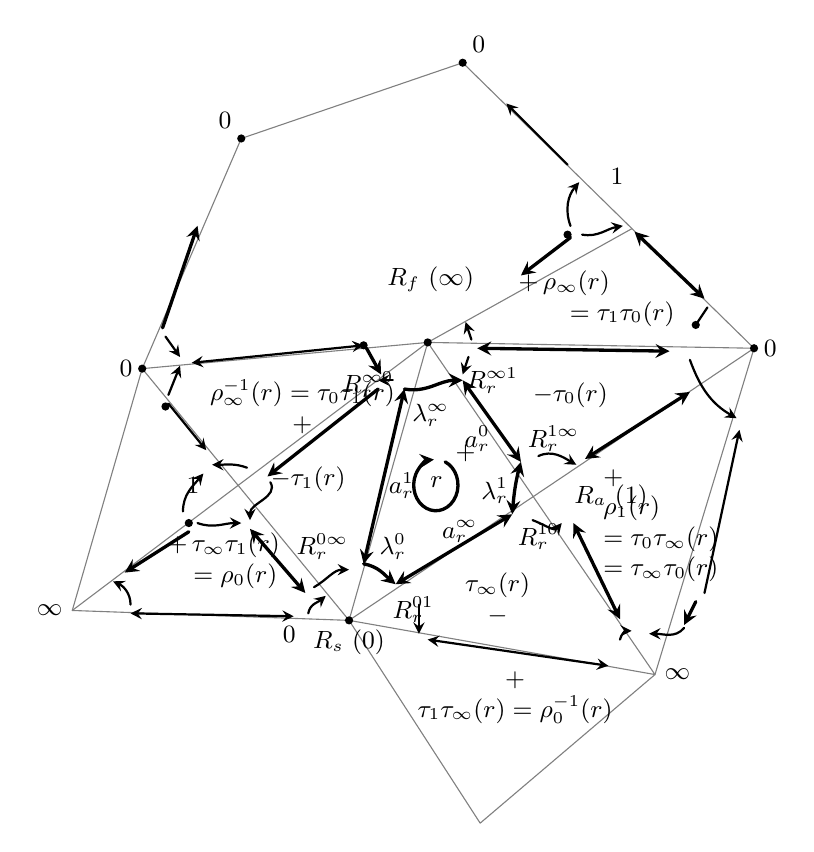
\begin{tikzpicture}[scale=.74,>=stealth,every node/.style={font=\small},line cap=round,line join=round]
\coordinate (T) at (7.5,-.6);
\coordinate (TL) at (3.7,-1.9);
\coordinate (L) at (2,-5.85);
\coordinate (LL) at (.8,-10);
\coordinate (F) at (6.9,-5.4);
\coordinate (S) at (5.55,-10.17);
\coordinate (A) at (9.5,-7.5);
\coordinate (TR) at (10.4,-3.45);
\coordinate (R) at (12.5,-5.5);
\coordinate (BR) at (10.8,-11.1);
\coordinate (B) at (7.8,-13.65);
\coordinate (AL) at (3.15,-7.5);
\draw[thin,gray] (TL)--(T)--(R)--(BR)--(B)--(S)--(LL)--(L)--cycle;
\draw[thin,gray] (L)--(S) (LL)--(F)--(R) (F)--(TR) (F)--(S) (F)--(BR) (S)--(R) (S)--(BR);
\draw[thin,gray] (L)--(F);
\foreach \p in {T,TL,L,F,S,R} \fill (\p) circle (2pt);
\node[above right] at (T) {$0$};
\node[above left] at (TL) {$0$};
\node[left] at (L) {$0$};
\node[left] at (LL) {$\infty$};
\node[right] at (R) {$0$};
\node[right] at (BR) {$\infty$};
\node[below] at (S) {$R_s\ (0)$};
\node[above] at (6.95,-4.7) {$R_f\ (\infty)$};
\node[right] at (9.25,-8.05) {$R_a\ (1)$};
\node[above] at (10.15,-2.85) {$1$};
\node[left] at (3.15,-7.85) {$1$};
\node[below left] at (4.8,-10.1) {$0$};
\draw[->,very thick] (2.35,-5.15)--(2.95,-3.4);
\draw[->,thick] (9.3,-2.35)--(8.25,-1.3);
\draw[<->,very thick] (10.45,-3.5)--(11.65,-4.65);
\draw[->,very thick] (9.35,-3.6)--(8.5,-4.25);
\draw[->,thick] (9.35,-3.4) to[out=110,in=230] (9.5,-2.65);
\draw[->,thick] (9.55,-3.55) to[out=-10,in=190] (10.25,-3.4);
\fill (9.3,-3.55) circle (2pt);
\fill (11.5,-5.1) circle (2pt);
\draw[thick] (11.7,-4.8)--(11.5,-5.1);
\draw[->,thick] (11.4,-5.7) to[out=-70,in=150] (12.2,-6.7);
\draw[->,thick] (11.65,-9.7)--(12.25,-6.9);
\draw[<->,very thick] (9.4,-8.5)--(10.2,-10.15);
\draw[->,thick] (10.2,-10.5) to[out=80,in=180] (10.4,-10.35);
\draw[->,thick] (11.3,-10.3) to[out=-130,in=0] (10.7,-10.4);
\draw[->,very thick] (11.5,-9.85)--(11.3,-10.25);
\draw[<->,thick] (6.9,-10.5)--(10,-10.95);
\draw[->,thick] (6.75,-9.9)--(6.75,-10.4);
\draw[<->,thick] (1.8,-10.05)--(4.6,-10.1);
\draw[->,thick] (1.8,-9.9) to[out=90,in=-25] (1.5,-9.5);
\draw[->,very thick] (2.8,-8.65)--(1.7,-9.35);
\fill (2.8,-8.5) circle (2pt);
\draw[->,thick] (2.7,-8.3) to[out=90,in=230] (3.05,-7.65);
\draw[->,thick] (2.95,-8.5) to[out=-20,in=180] (3.7,-8.5);
\draw[->,thick] (4.2,-7.8) to[out=-60,in=90] (3.85,-8.45);
\draw[->,thick] (3.8,-7.55) to[out=160,in=0] (3.2,-7.5);
\draw[<->,very thick] (3.85,-8.6)--(4.8,-9.7);
\draw[->,thick] (4.85,-10.05) to[out=80,in=-140] (5.15,-9.75);
\draw[->,thick] (4.95,-9.6) to[out=30,in=180] (5.55,-9.3);
\draw[->,thick] (2.45,-6.45)--(3.1,-7.25);
\fill (2.4,-6.5) circle (2pt);
\draw[->,thick] (2.45,-6.3)--(2.65,-5.8);
\draw[->,thick] (2.4,-5.3)--(2.65,-5.65);
\draw[<->,thick] (2.85,-5.75)--(5.8,-5.45);
\fill (5.8,-5.45) circle (2pt);
\draw[->,very thick] (5.85,-5.5)--(6.1,-5.95);
\draw[->,thick] (6.3,-6.05)--(6.05,-6.05);
\draw[->,very thick] (6.05,-6.2)--(4.15,-7.7);
\draw[<->,very thick] (7.75,-5.5)--(11.05,-5.55);
\draw[->,thick] (7.65,-5.35)--(7.55,-5.05);
\draw[->,thick] (7.6,-5.65)--(7.5,-5.95);
\draw[<->,very thick] (9.6,-7.4)--(11.4,-6.25);
\draw[->,thick] (8.8,-7.35) to[out=25,in=150] (9.45,-7.5);
\draw[->,thick] (8.7,-8.45) to[out=-20,in=230] (9.2,-8.5);
\coordinate (F0) at (6.5,-6.2);
\coordinate (F1) at (7.5,-6.05);
\coordinate (Ainf) at (8.5,-7.45);
\coordinate (A0) at (8.35,-8.35);
\coordinate (S1) at (6.35,-9.55);
\coordinate (Sinf) at (5.8,-9.2);
\draw[<->,very thick] (Sinf)--(F0);
\draw[->,very thick] (F0) to[out=-10,in=180] (F1);
\draw[<->,very thick] (F1)--(Ainf);
\draw[<->,very thick] (Ainf) to[out=-105,in=85] (A0);
\draw[<->,very thick] (A0)--(S1);
\draw[->,very thick] (Sinf) to[out=-10,in=140] (S1);
\draw[->,very thick] (7.2,-7.45) arc[start angle=65,end angle=-265,x radius=.38,y radius=.44];
\node at (7.05,-7.8) {$r$};
\node at (7.55,-7.3) {$+$};
\node at (6.45,-7.85) {$a_r^1$};
\node at (7.75,-7.05) {$a_r^0$};
\node at (7.45,-8.65) {$a_r^\infty$};
\node at (6.95,-6.65) {$\lambda_r^\infty$};
\node at (8.05,-7.95) {$\lambda_r^1$};
\node at (6.3,-8.9) {$\lambda_r^0$};
\node[anchor=east] at (6.48,-6.12) {$R_r^{\infty 0}$};
\node[anchor=west] at (7.4,-6.05) {$R_r^{\infty 1}$};
\node[anchor=west] at (8.45,-7.05) {$R_r^{1\infty}$};
\node[anchor=north] at (8.8,-8.35) {$R_r^{10}$};
\node[anchor=east] at (5.7,-8.9) {$R_r^{0\infty}$};
\node[anchor=north] at (6.65,-9.6) {$R_r^{01}$};
\node at (4.85,-7.75) {$-\tau_1(r)$};
\node at (9.35,-6.3) {$-\tau_0(r)$};
\node[align=center] at (8.1,-9.8) {$\tau_\infty(r)$\\$-$};
\node[align=center] at (4.75,-6.5) {$\rho_\infty^{-1}(r)=\tau_0\tau_1(r)$\\$+$};
\node[align=left] at (9.8,-4.65) {$+\,\rho_\infty(r)$\\$\qquad=\tau_1\tau_0(r)$};
\node[align=left] at (3.4,-9.15) {$+\,\tau_\infty\tau_1(r)$\\$\quad=\rho_0(r)$};
\node[align=center] at (8.4,-11.5) {$+$\\$\tau_1\tau_\infty(r)=\rho_0^{-1}(r)$};
\node[align=left] at (10.9,-8.55) {$+$\\$\unsure{\rho_1(r)}$\\$=\tau_0\tau_\infty(r)$\\$=\tau_\infty\tau_0(r)$};
\end{tikzpicture}}

\[
 (2)\quad
 \left\{\begin{aligned}
 \tau_\infty\tau_1(r)&=\rho_0(r)\\
 \tau_1\tau_\infty(r)&=\rho_0^{-1}(r)
 \end{aligned}\right.
 \qquad\text{(sommet conservé)}
\]
où $\rho_0$ est la rotation \inserted{d'un cran} autour du sommet de type $0$, dans le sens indiqué par l'orientation choisie pour $r$. Enfin
\[
 (3)\qquad\tau_0\tau_\infty(r)=\tau_\infty\tau_0(r)\overset{\mathrm{def}}=\rho_1(r),
\]

[ Pour mémoire, les relations dans le groupe cartographique
\[
 (4)\qquad\tau_0^2=\tau_1^2=\tau_\infty^2=(\tau_0\tau_\infty)^2=1
\]
\[
 (5)\quad
 \left\{\begin{aligned}
 \rho_\infty&=\tau_1\tau_0\\
 \rho_0&=\tau_\infty\tau_1\\
 \rho_1&=\tau_0\tau_\infty
 \end{aligned}\right.
 \qquad\rho_\infty\rho_1\rho_0\deleted{\unsure{\rho_\infty}}=1
 \qquad\text{]}
\]
\mspage{113}
